\documentclass{standalone}
\usepackage{tikz}
\usetikzlibrary{positioning}
\usetikzlibrary{calc}
\usetikzlibrary{decorations.pathreplacing}

\begin{document}

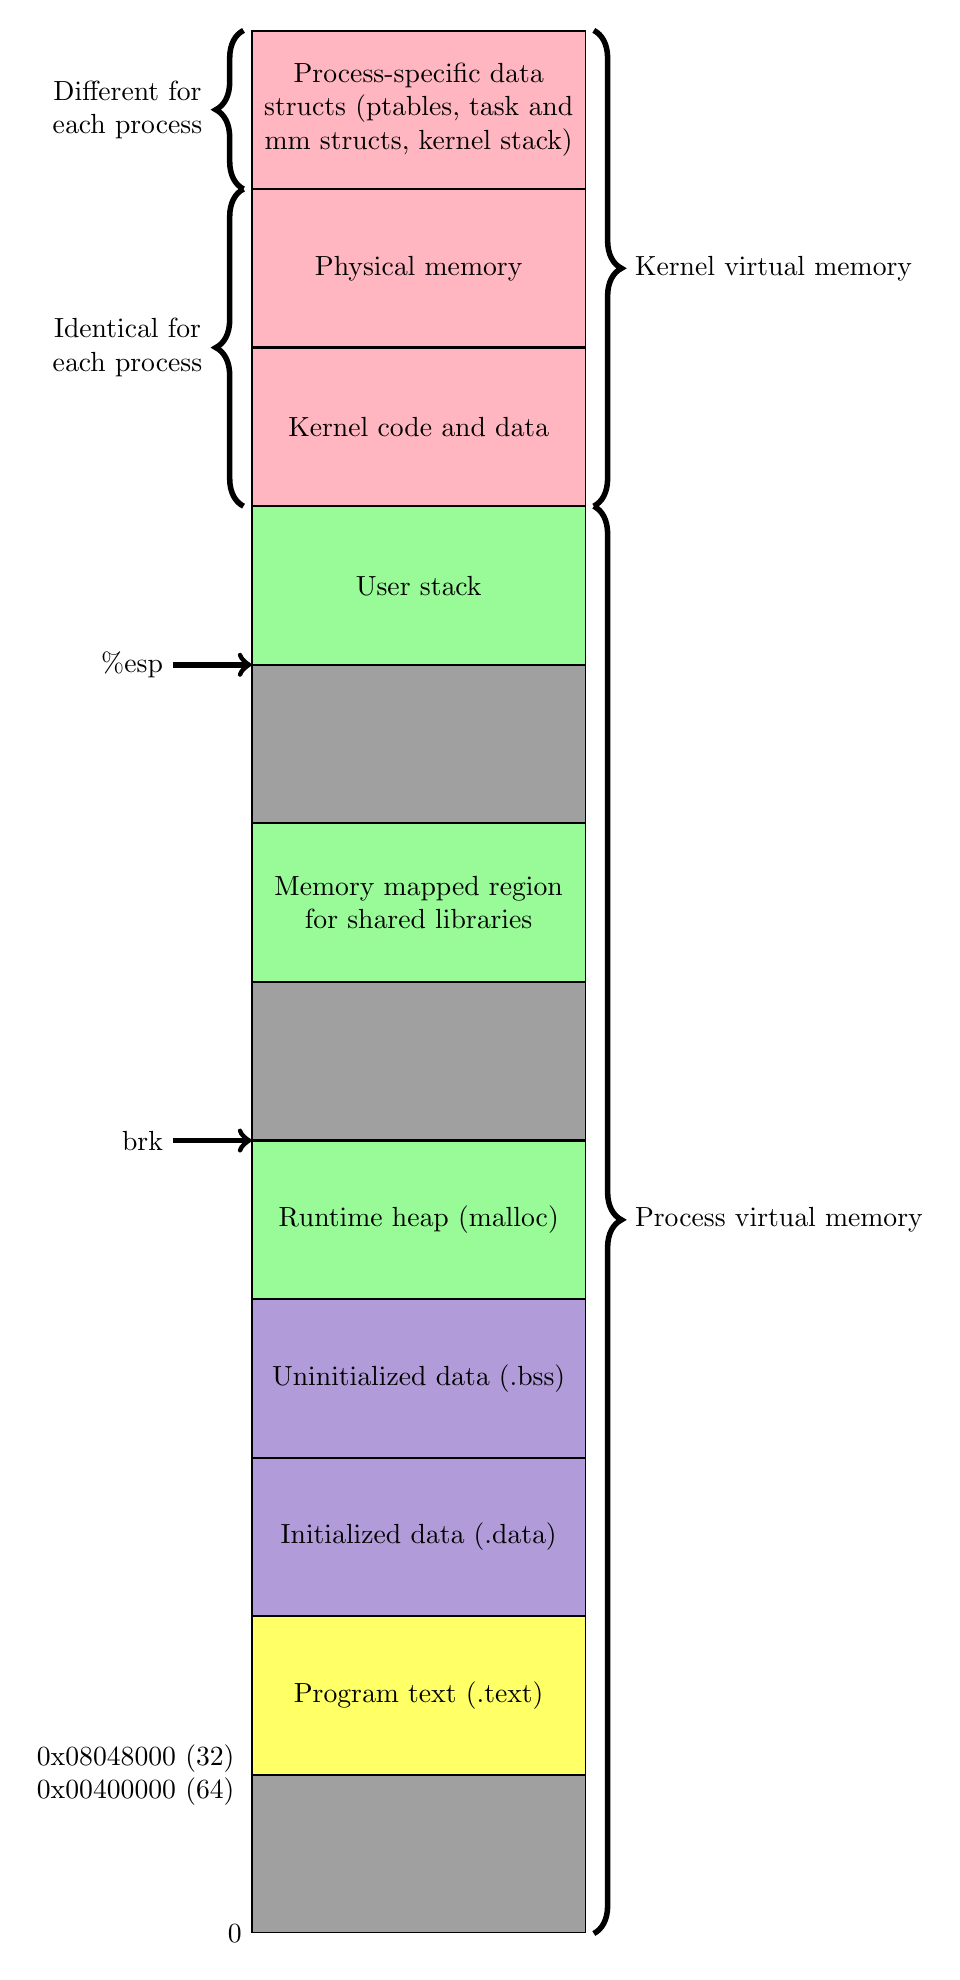
\begin{tikzpicture}

% Define colors
\definecolor{programtext}{RGB}{255,255,102}
\definecolor{initdata}{RGB}{177,156,217}
\definecolor{uninitdata}{RGB}{177,156,217}
\definecolor{runtimeheap}{RGB}{152,251,152}
\definecolor{mmapregion}{RGB}{152,251,152}
\definecolor{userstack}{RGB}{152,251,152}
\definecolor{kerneldata}{RGB}{255,182,193}
\definecolor{physicalmem}{RGB}{255,182,193}
\definecolor{processdata}{RGB}{255,182,193}
\definecolor{empty-gray}{RGB}{160,160,160}

% Node style
\tikzset{
    memblock/.style={draw, rectangle, align=center, text width=4cm, minimum height=2cm, minimum width=4cm},
    label/.style={
        anchor=east
    }
}

% Place nodes
\node[memblock, fill=empty-gray] (empty-1) {};
\node[memblock, fill=programtext,above=0cm of empty-1] (text) {Program text (.text)};
\node[memblock, fill=initdata, above=0cm of text] (data) {Initialized data (.data)};
\node[memblock, fill=uninitdata, above=0cm of data] (bss) {Uninitialized data (.bss)};
\node[memblock, fill=runtimeheap, above=0cm of bss] (heap) {Runtime heap (malloc)};
\node[memblock, fill=empty-gray,above=0cm of heap] (empty-2) {};
\node[memblock, fill=mmapregion, above=0cm of empty-2] (mmap) {Memory mapped region for shared libraries};
\node[memblock, fill=empty-gray,above=0cm of mmap] (empty-3) {};
\node[memblock, fill=userstack, above=0cm of empty-3] (stack) {User stack};
\node[memblock, fill=kerneldata, above=0cm of stack] (kernel) {Kernel code and data};
\node[memblock, fill=physicalmem, above=0cm of kernel] (physical) {Physical memory};
\node[memblock, fill=processdata, above=0cm of physical] (process) {Process-specific data structs (ptables, task and mm structs, kernel stack)};


% Labels
\node[label] at ($(empty-1.south west) + (-0.0, 0)$) {0};
\node[label, text width = 3cm,minimum width = 3cm,minimum height = 3cm] at ($(text.south west) + (+0.4, 0)$) {0x08048000 (32)\\0x00400000 (64)};
\node[label] at ($(heap.north west) + (-1.0, 0)$) (brk) {brk};
\node[label] at ($(stack.south west) + (-1.0, 0)$) (esp) {\%esp};

\node[align=left,anchor=west] at ($(heap.east) + (+0.5, 0)$) {Process virtual memory};
\node[align=left,anchor=west] at ($(physical.east) + (+0.5, 0)$) {Kernel virtual memory};
\node[align=center,anchor=east] at ($(process.west) + (-0.5, 0)$) {Different for\\each process};
\node[align=center,anchor=east] at ($(kernel.north west) + (-0.5, 0)$) {Identical for\\each process};

% Left big parenthesis
\draw[line width=2pt, decorate,decoration={brace,amplitude=10pt}] ($(process.north east) + (0.1,0)$) -- ($(kernel.south east) + (0.1,0)$);
\draw[line width=2pt, decorate,decoration={brace,amplitude=10pt}] ($(stack.north east) + (0.1,0)$) -- ($(empty-1.south east) + (0.1,0)$);

% Right big parenthesis
\draw[line width=2pt, decorate,decoration={brace,mirror,amplitude=10pt}] ($(process.north west) + (-0.1, 0)$) -- ($(process.south west) + (-0.1, 0)$);
\draw[line width=2pt, decorate,decoration={brace,mirror,amplitude=10pt}] ($(physical.north west) + (-0.1, 0)$)-- ($(kernel.south west) + (-0.1, 0)$);

\draw[line width=2pt, ->] (brk.east) -- (heap.north west);
\draw[line width=2pt, ->] (esp.east) -- (stack.south west);

\end{tikzpicture}
\end{document}


